\documentclass[../report.tex]{subfiles}

\begin{document}

\subsection{Story and Narrative}
Trò chơi nói về viễn cảnh của trái đất vào những
năm 2500 khi bị các quái vật ngoài hành tinh xâm chiếm.
Lực lượng quân đội trái đất đã tạo ra những Robot
để có khả năng chống lại sự xâm chiếm của các quái vật đó.
Mỗi Robot được thiết kế với một khẩu súng LASER có
thể tiêu diệt nhanh chóng các quái vật. 

\subsection{Game World}
\subsubsection{General look and feel of world}
\begin{itemize}
\item Không có
\end{itemize}

\subsubsection{Areas}
\begin{itemize}
\item Không có
\end{itemize}

\subsection{Characters}
\subsubsection{Player (Hero)}
\begin{itemize}
\item Hình ảnh:
\begin{figure}[H]
\centering
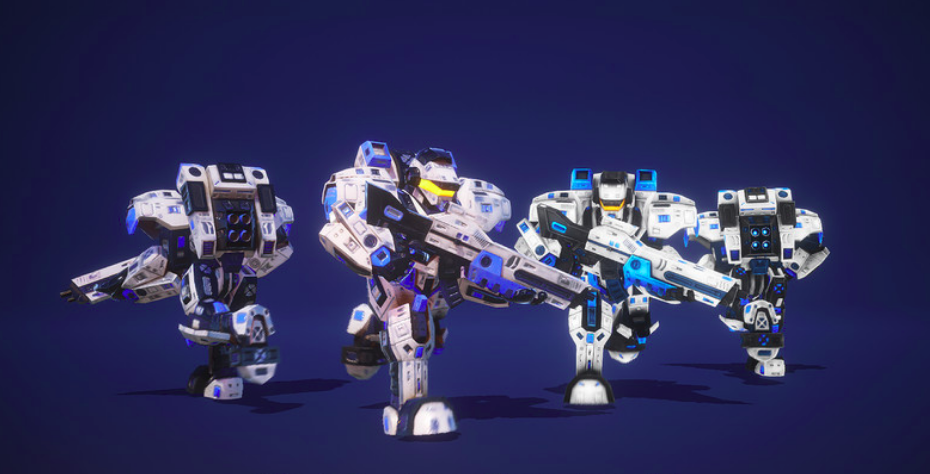
\includegraphics[width=15cm]{figures/hero.png}
\end{figure}

\item Di chuyển: sang trái, sang phải,
tiến lên, lùi lại , quay quay đầu
\item Hành động: Bắn đạn (Kèm hiệu ứng hình ảnh + âm thanh)
\item Đạn: Tia laze
\end{itemize}

\subsubsection{Enemy}
\paragraph{Voi}

\begin{itemize}
\item Hình ảnh:
\begin{figure}[H]
\centering
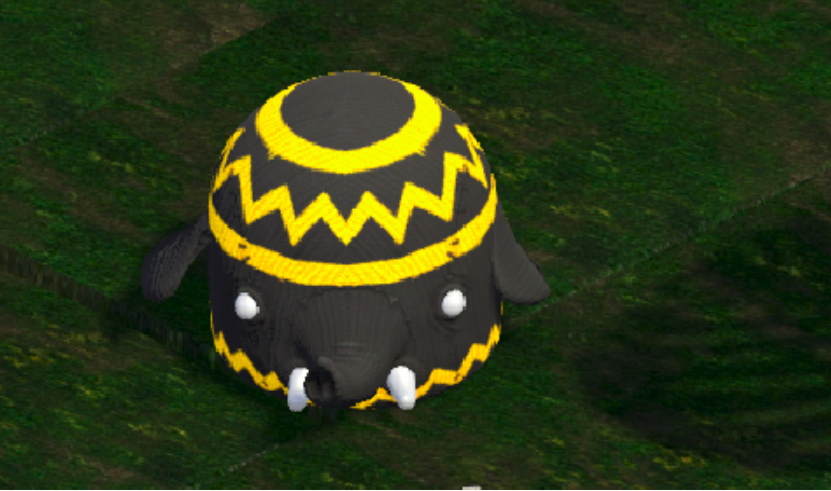
\includegraphics[width=13cm]{figures/voi.png}
\end{figure}

\item Di chuyển: Di chuyển tự do trên màn
\item hành động: Băn đạn tấn sát thương player theo 2 kiểu: bắn thắng và bắn vòng tròn lan tỏa về mọi hướng
\item Đạn: 
\begin{figure}[H]
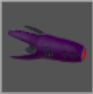
\includegraphics[width=3cm]{figures/voi-dan.png}
\end{figure}
\end{itemize}

\paragraph{Nhện}

\begin{itemize}
\item Hình ảnh:
\begin{figure}[H]
\centering
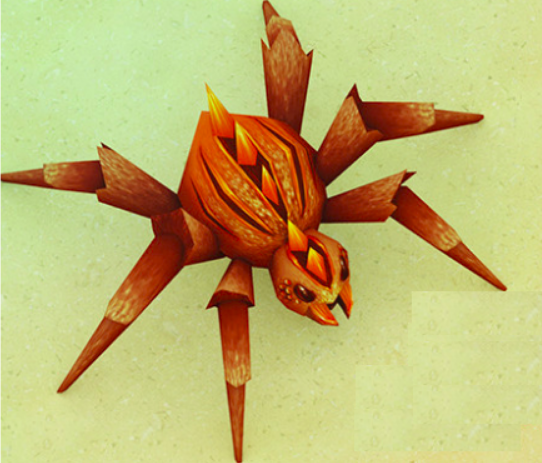
\includegraphics[width=9cm]{figures/nhen.png}
\end{figure}

\item Di chuyển: Tự do di chuyển trên map 
\item Hành động: tấn công khi áp sát player

\end{itemize}

\paragraph{Zoombear}
\begin{itemize}
\item Hình ảnh:
\begin{figure}[H]
\centering
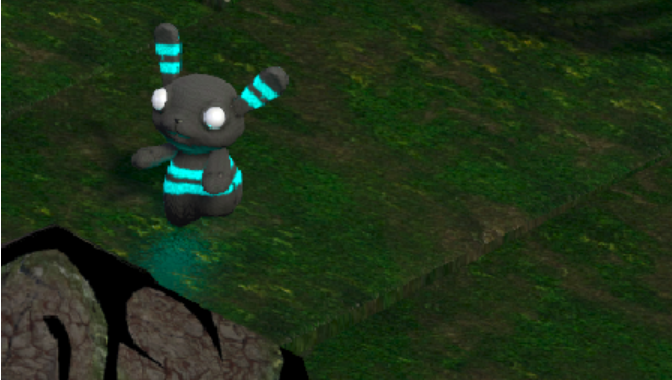
\includegraphics[width=9cm]{figures/zoombear.png}
\end{figure}

\item Di chuyển: Tự do di chuyển trên map 
\item Hành động: tấn công khi áp sát player
\end{itemize}

\paragraph{Bọ cạp}
\begin{itemize}
\item Hình ảnh:
\begin{figure}[H]
\centering
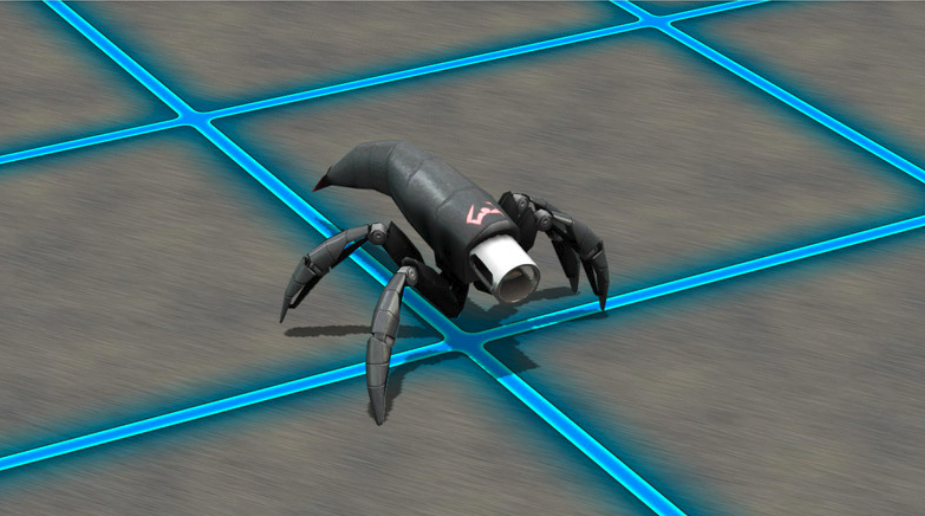
\includegraphics[width=12cm]{figures/bocap.png}
\end{figure}

\item Di chuyển: Tự do di chuyển trên map
\item hành động: Sát thương bằng bullet và khi áp sát
\item Đạn LASER
\end{itemize}

\end{document}
